\documentclass{article}
\usepackage[UTF8]{ctex}
\usepackage{geometry}
\usepackage{makecell}
\usepackage{amsmath}
\usepackage{graphicx}
\usepackage{subcaption}

\geometry{a4paper,scale=0.75}

\title{\heiti 实验十六\ 霍尔效应测量磁场}
\author{\kaishu 田睿轩\ 物理学院\ 1900011602}
\date{2020年11月20日}
\newcommand{\degree}{^\circ}

\begin{document}
    \maketitle
    \section{数据处理}
    \subsection{测量$U_H$与$I_H$的关系}
    如图所示搭建电路

    \begin{center}
        \includegraphics[width=0.4\textwidth]{dianlutu.jpg}  
    \end{center}
    
    实验中控制励磁电流$I_M=0.600A$大小不变,从而控制磁场$B$不变,改变$I_H$,
    研究霍尔电压$U_H$与电流$I_H$的关系。

    为了消除负效应,对同一大小的$I_H$,改变$I_H$与$B$的方向,分别测量$U_H$的大小。

    实验中,$U_1$对应的方向为:$I:+,B:+$,$U_2$对应的方向为:$I:-,B:+$,
    $U_3$对应的方向为:$I:-,B:-$,$U_1$对应的方向为:$I:+,B:-$,
    $U=\frac{1}{4}(U_1-U_2+U_3-U_4)$。

    为了研究霍尔片几何结构对霍尔电压的影响,分别将电流从1、2端和3、4端输入。

    \subsubsection{电流从1、2端输入}

    实验数据如下表所示:
    \begin{center}
        \begin{tabular}{|c|c|c|c|c|c|}
            \hline
            $I_M(mA)$ & $U_1(mV)$ & $U_2(mV)$ & $U_3(mV)$ & $U_4(mV)$ & $U(mV)$ \\
            \hline
            2.000 & 4.86 & -4.85 & 4.95 & -4.94 & 4.90\\
            \hline
            4.000 & 9.72 & -9.71 & 9.89 & -9.89 & 9.80\\
            \hline
            6.000 & 14.59 & -14.58 & 14.85 & -14.84 & 14.72\\
            \hline
            8.000 &  19.47 & -19.46 & 19.80 & -19.80 & 19.63\\
            \hline
            10.000 & 24.36 & -24.35 & 24.77 & -24.76 & 24.56\\
            \hline
        \end{tabular}        
    \end{center}

    根据实验数据绘制$U_H-I_H$曲线,如下图所示:

    \begin{center}
        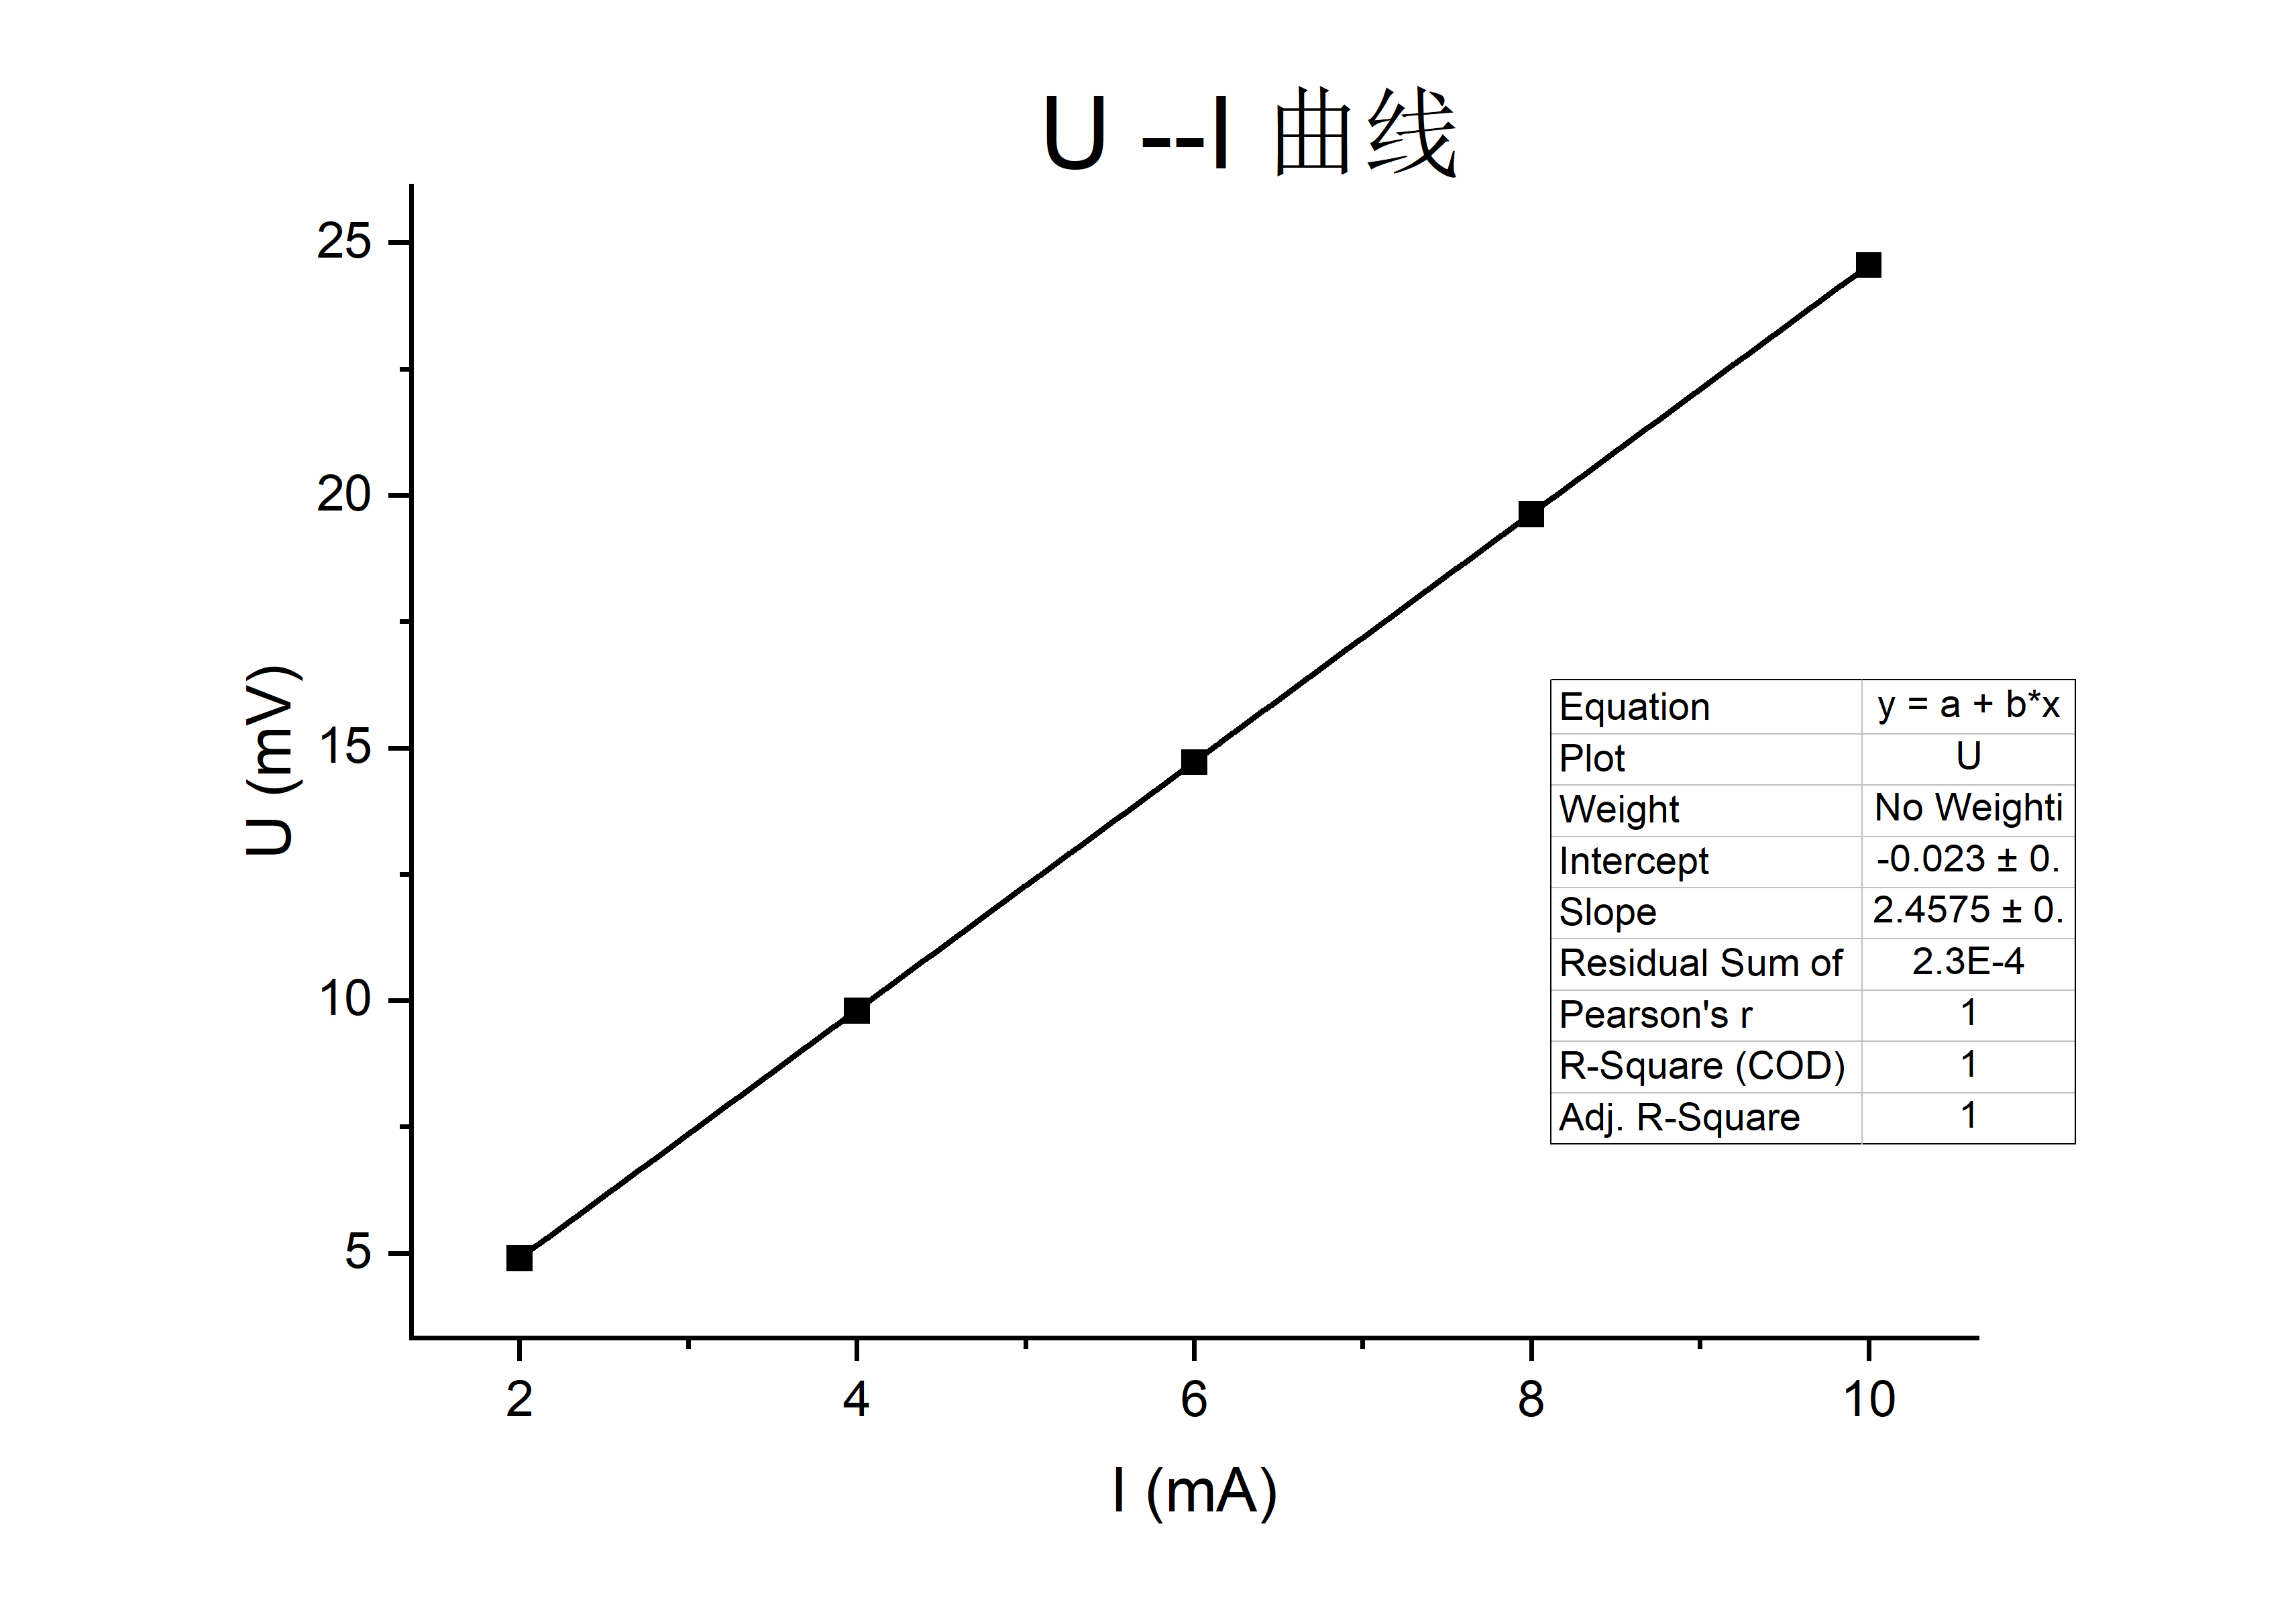
\includegraphics[width=0.8\textwidth]{U-I curve.jpg}
    \end{center}

    \subsubsection{电流从3、4端输入}

    实验数据如下表所示:

    \begin{center}
        \begin{tabular}{|c||c|c|c|c||c|}
            \hline
            $I_M(mA)$ & $U_1(mV)$ & $U_2(mV)$ & $U_3(mV)$ & $U_4(mV)$ & $U(mV)$ \\
            \hline
            2.000 & 4.93 & -4.98 & 4.84 & -4.90 & 4.91\\
            \hline
            4.000 & 9.88 & -9.93 & 9.71 & -9.77 & 9.82\\
            \hline
            6.000 & 14.84 & -14.89 & 14.59 & -14.64 & 14.74\\
            \hline
            8.000 &  19.80 & -19.85 & 19.47 & -19.52 & 19.66\\
            \hline
            10.000 & 24.77 & -24.81 & 24.36 & -24.40 & 24.58\\
            \hline
        \end{tabular}        
    \end{center}

    根据实验数据绘制$U_H-I_H$曲线,如下图所示:

    \begin{center}
        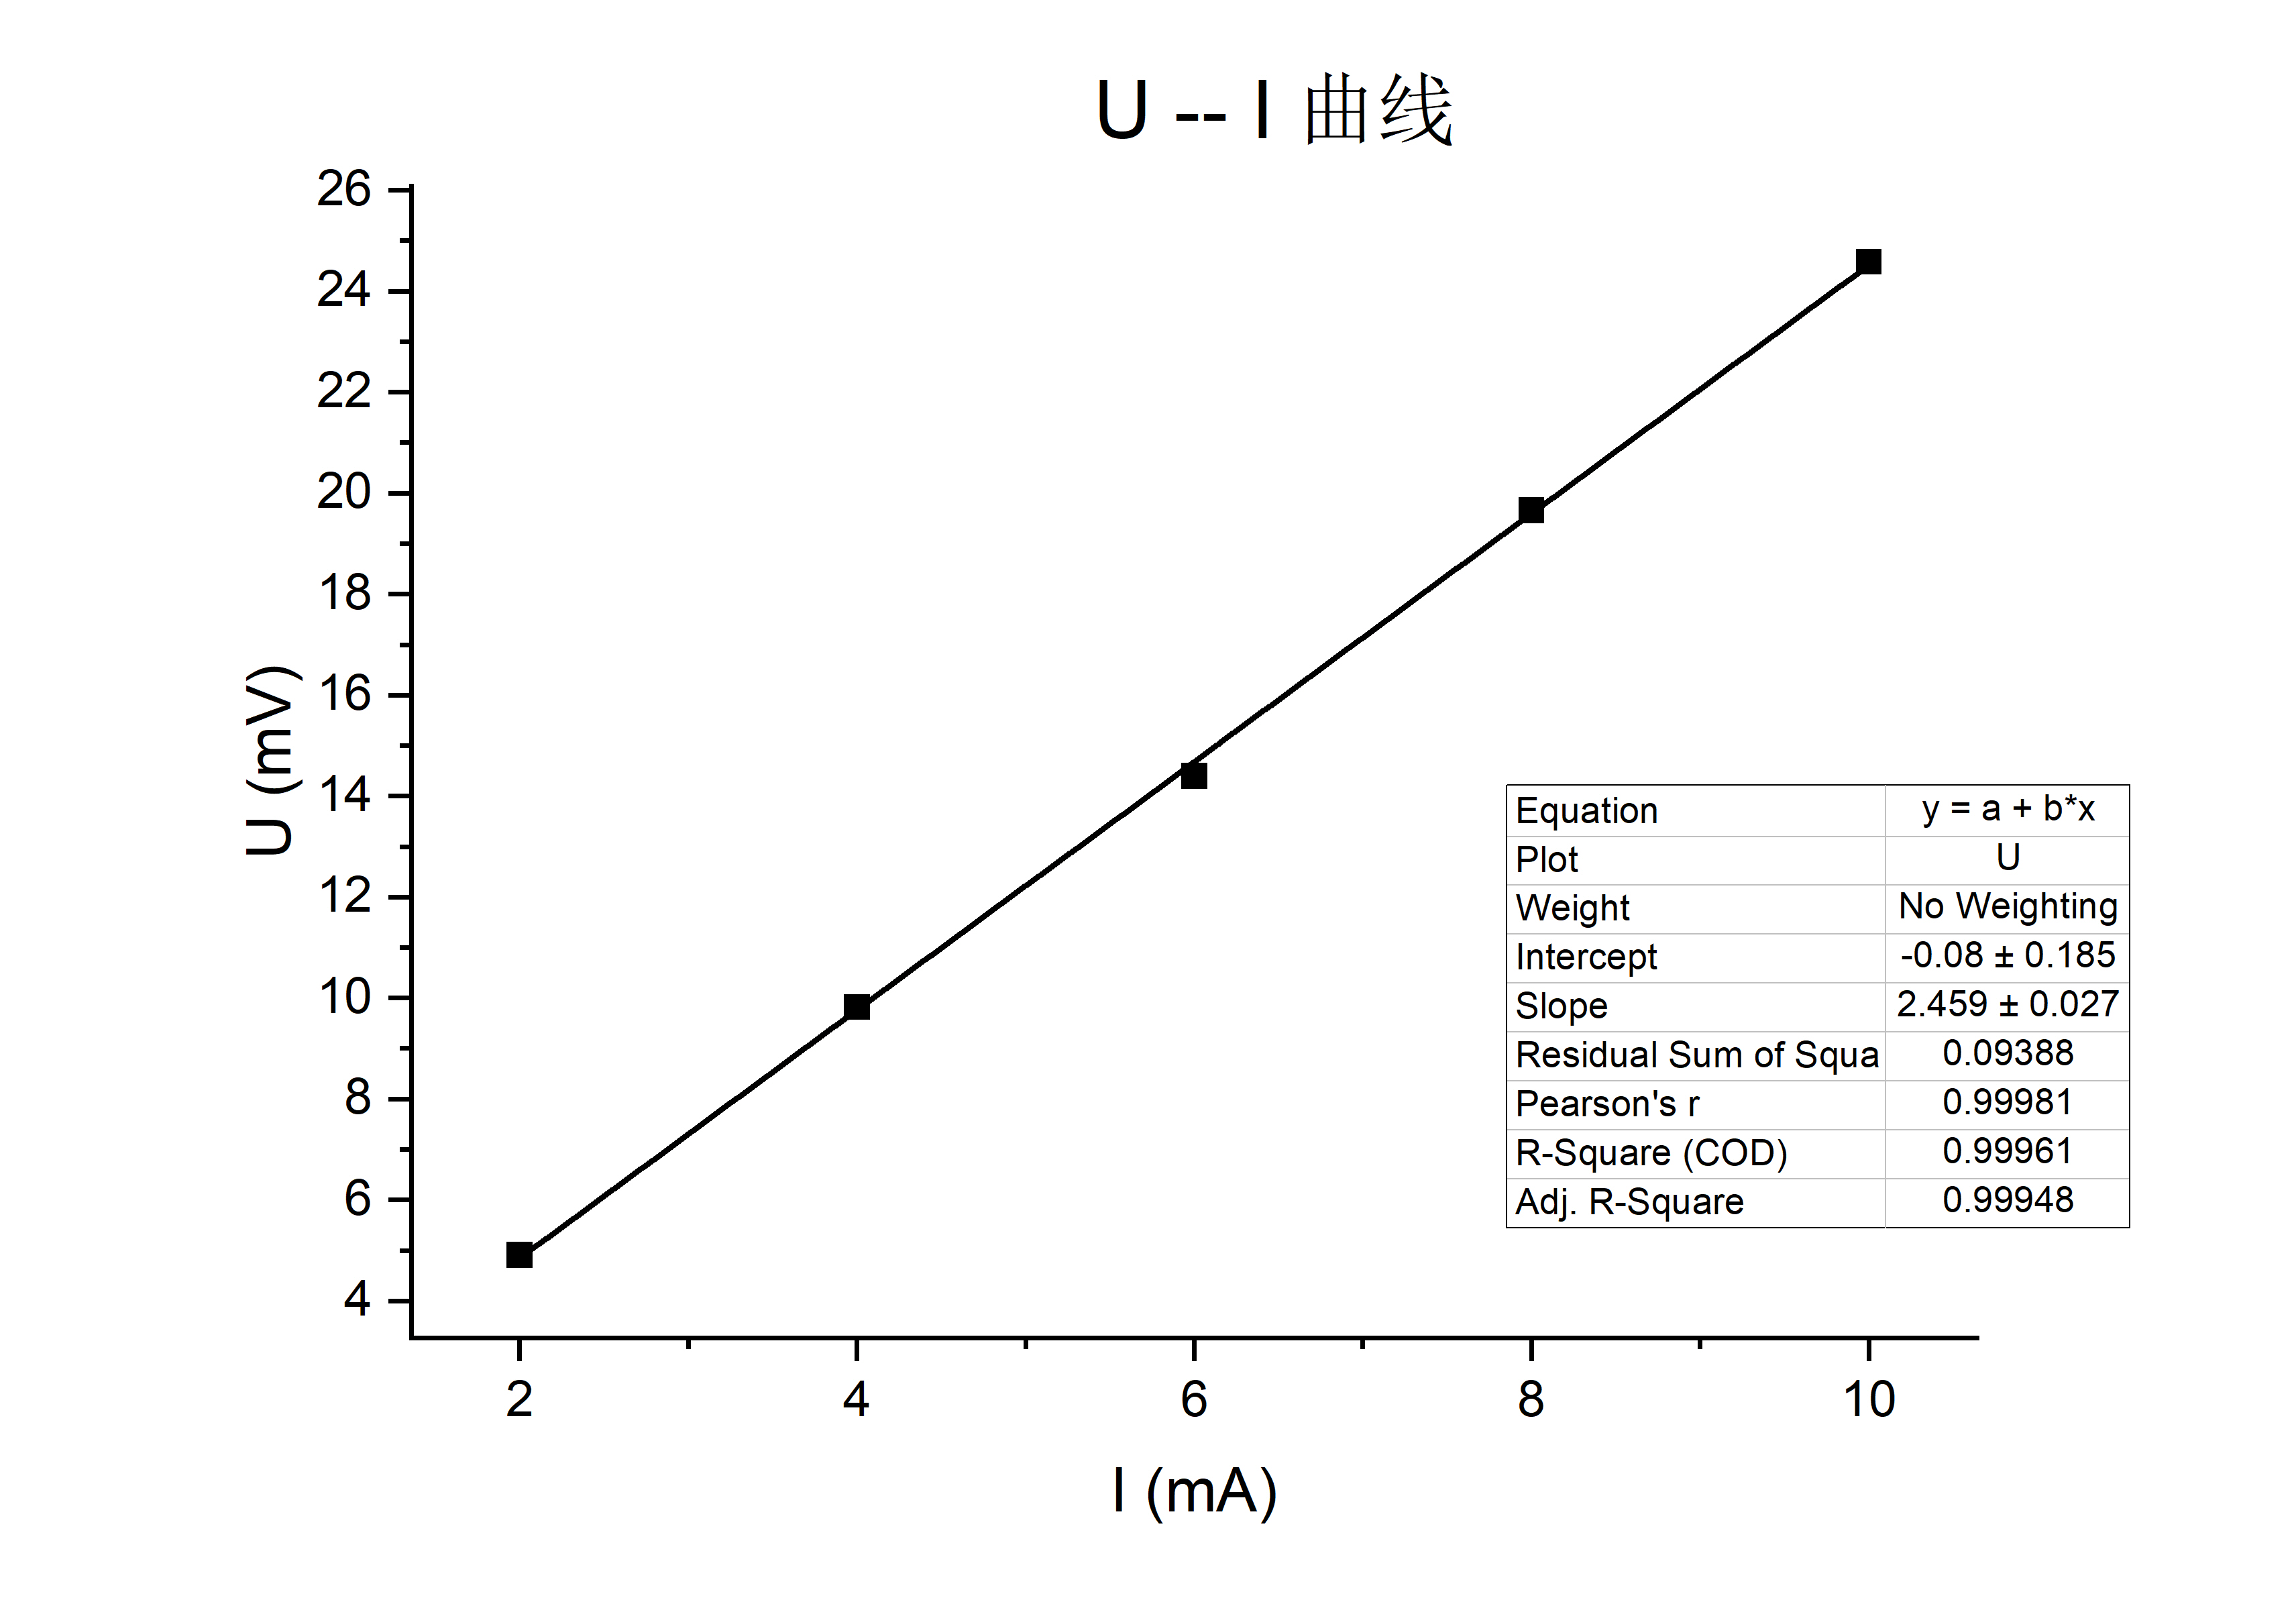
\includegraphics[width=0.8\textwidth]{U-I curve2.jpg}
    \end{center}

    比较电流从1、2端流入和从3、4端流入的数据,可以看出:

    同一接法下,$U_1,U_2,U_3,U_4$的绝对值基本相等,但仍然可以发现有因负效应带来的差异;
    不同接法下,$U_1,U_2,U_3,U_4$有一定差别,但消除负效应后的$U$基本相等。
    可见霍尔片的长、宽对霍尔电压的大小无影响。

    \subsection{测量$U_H$与$B$的关系并计算$K_H$}
    保持霍尔电流$I_H=10.00mA$不变,改变励磁电流$I_M$的大小,测量霍尔电压$U_H$的大小,并用特斯拉计霍尔片所在
    位置磁场$B$的大小,研究$U_H$与$B$的关系。

    实验数据如下表所示:

    \begin{center}
        \begin{tabular}{|c||c||c|c|c|c||c|}
            \hline
            $I_M(mA)$ & $B(mT)$ &$U_1(mV)$ & $U_2(mV)$ & $U_3(mV)$ & $U_4(mV)$ & $U(mV)$ \\
            \hline
            0.000 & 1.0 & -0.11 & 0.13 & 0.12 & -0.10 & -0.01 \\
            \hline
            0.100 & 36.0 & 3.69 & -3.68 & 4.15 & -4.14 & 3.92 \\
            \hline
            0.200 & 74.9 & 7.89 & -7.89 & 8.38 & -8.37 & 8.13 \\
            \hline
            0.300 & 112.0 & 12.08 & -12.08 & 12.48 & -12.48 & 12.28 \\
            \hline
            0.400 & 151.1 & 16.18 & -16.18 & 16.59 & -16.59 & 16.38 \\
            \hline
            0.500 & 189.0 & 20.23 & -20.22 & 20.72 & -20.72 & 20.47 \\
            \hline
            0.600 & 226.3 & 24.36 & -24.36 & 24.78 & -24.78 & 24.57 \\
            \hline
            0.700 & 266.4 & 28.37 & -28.37 & 28.80 & -28.80 & 28.58 \\
            \hline
            0.800 & 298.6 & 32.27 & -32.27 & 32.78 & -32.77 & 32.52 \\
            \hline
            0.900 & 336.6 & 36.23 & -36.23 & 36.66 & -36.66 & 36.44 \\
            \hline
            1.000 & 370.4 & 40.01 & -40.00 & 40.45 & -40.43 & 40.22 \\
            \hline
        \end{tabular}        
    \end{center}

    绘制$U_H-B$曲线,如下图所示:

    \begin{center}
        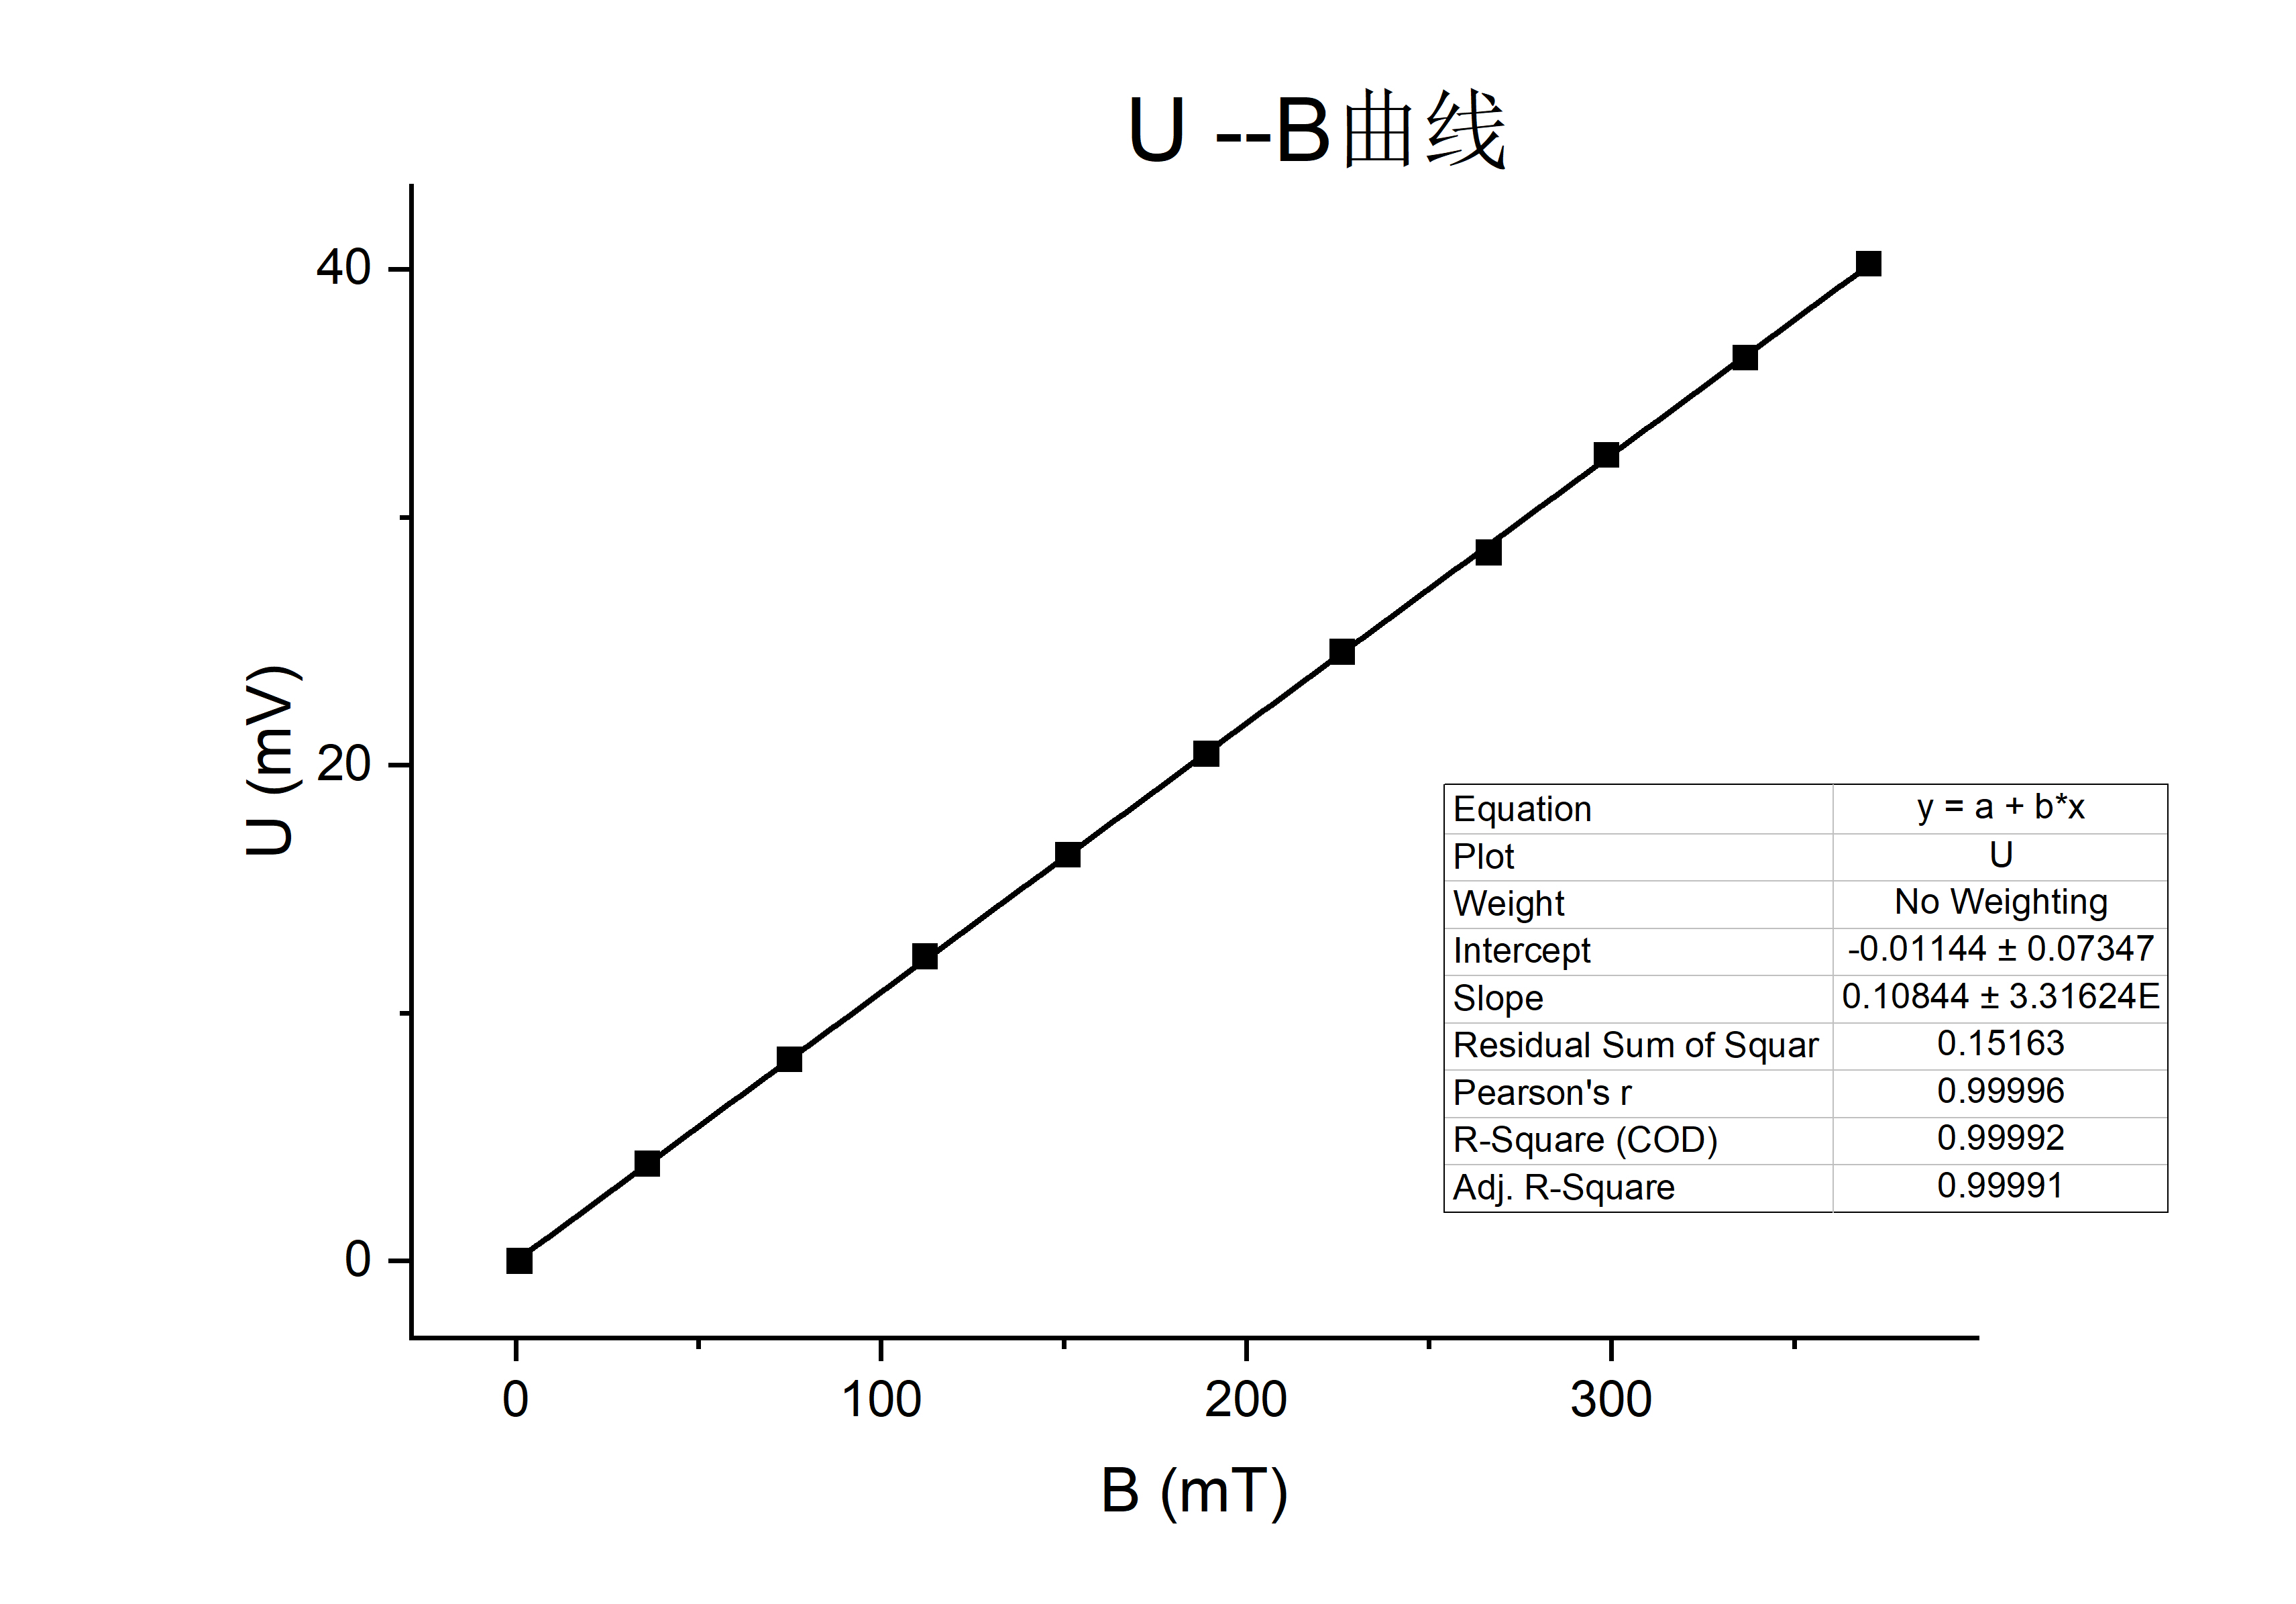
\includegraphics[width=0.8\textwidth]{U-B curve.jpg}
    \end{center}

    曲线斜率$a=108.4mV/T$,截距$b=-0.0114mV$,相关系数$r=0.99996$。

    根据霍尔电压的表达式:$U_H=K_H I_H B=aB$,可以求出霍尔元件的灵敏度:
    $$K_H=\frac{a}{I_H}=10.84mV/(mA\cdot T)$$

    下面计算霍尔元件灵敏度$K_H$的不确定度:
    $$\sigma_{a,A}=a\sqrt{\frac{1/r^2-1}{n-2}}=108.4\sqrt{\frac{1/0.99996^2-1}{11-2}}=0.32mV/T$$
    $$\sigma_{a,B}=\frac{\sigma_U}{\sqrt{\sum_{i=1}^{11} (x_i-\bar{x})^2}}=\frac{(0.05\%\times40.22+0.03)/\sqrt{3}}{\sqrt{153195.61}\times 10^{-3}}=0.074mV/T$$
    $$\sigma_a=\sqrt{\sigma_{a,A}^2+\sigma_{a,B}^2}=0.33mV/T$$
    $$\sigma_{I_H}=\frac{e_I}{\sqrt{3}}=\frac{1.5\%\times 10.00+0.03}{\sqrt{3}}=0.104mA$$
    $$\sigma_{K_H}=K_H\sqrt{(\frac{\sigma_a}{a})^2+(\frac{\sigma_{I_H}}{I_H})^2}=10.84\times \sqrt{(\frac{0.33}{108.4})^2+(\frac{0.104}{10})^2}=0.12mV/(mA\cdot T)$$

    由此可得:
    $$H_H=(10.84\pm 0.12)mV/(mA\cdot T)$$

    \subsection{测量$B$与$I_M$关系}
    根据实验中测得的$U_H,I_H$和计算出的$K_H$计算不同励磁电流$I_M$下的磁感应强度大小$B$,
    并研究$B$与$I_M$关系。实验测得和计算所得数据如下表所示:

    $I_H=10.00mA,K_H=10.84mV/(mA\cdot T),B=\frac{U_H}{K_H\cdot I_H}$

    \vspace{1ex}
    \begin{tabular}{|c|c|c|c|c|c|c|c|c|c|c|c|}
        \hline
        $I_M(mA)$ & 0.000 & 0.100 & 0.200 & 0.300 & 0.400 & 0.500 & 0.600 & 0.700 & 0.800 & 0.900 & 1.000\\
        \hline
        $U_H(mV)$ & -0.01 & 3.92 & 8.13 & 12.28 & 16.38 & 20.47 & 24.57 & 28.58 & 32.52 & 36.44 & 40.22\\
        \hline
        $B(mT)$ & 0.0 & 36.1 & 75.0 & 113.3 & 151.2 & 189.9 & 226.7 & 263.7 & 300.0 & 336.2 & 371.1\\
        \hline
    \end{tabular}
    \vspace{1ex}
    
    根据数据绘制$B-I_M$磁化曲线:
    \begin{center}
        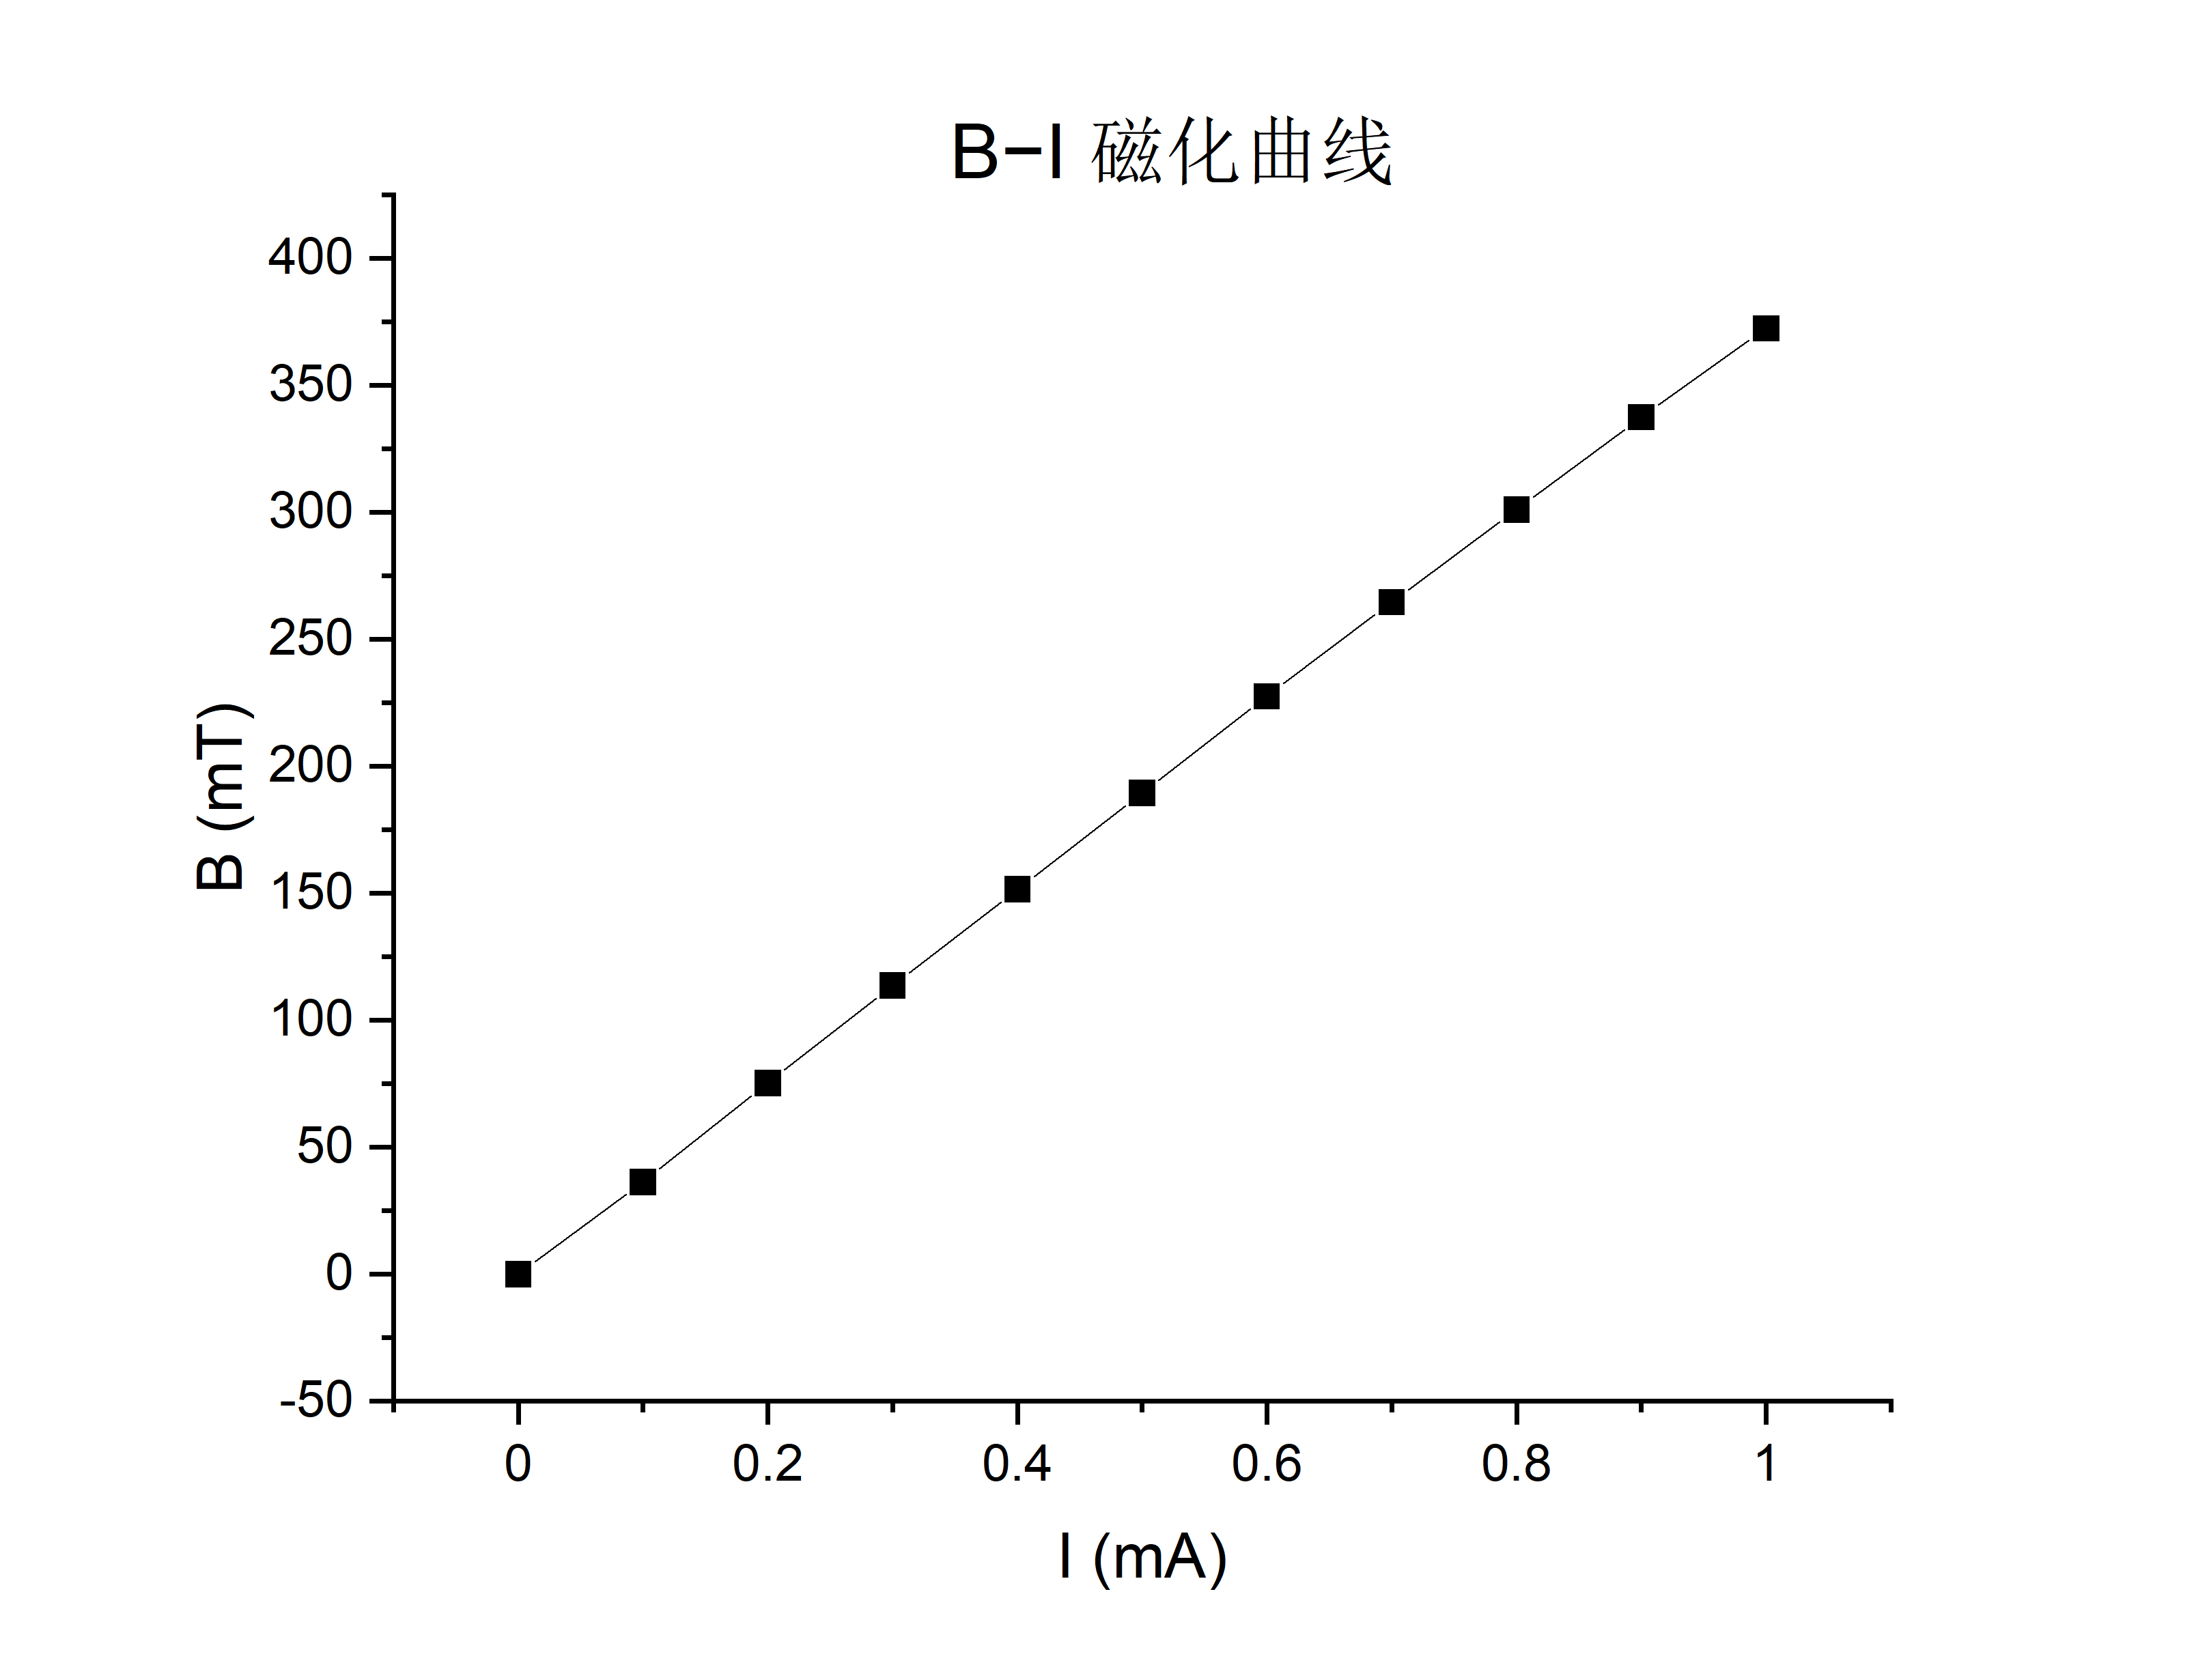
\includegraphics[width=0.8\textwidth]{B-I curve.jpg}
    \end{center}

    根据数据和图线可以看出,电磁铁产生的磁感应强度大小与励磁电流大小线性关系,可以判断材料为软磁材料。

    \subsection{测量电磁铁磁场沿水平方向分布}
    水平移动霍尔片,改变磁场相对霍尔片的位置,根据霍尔片上的霍尔电压计算霍尔片所处位置的磁场,
    从而获得磁场位置随坐标的分布。

    实验数据如下表所示:

    \vspace{1ex}
    \begin{tabular}{|c|c|c|c|c|c|c|c|c|c|c|c|}
        \hline
        $x(mm)$ & 70.0 & 69.0 & 68.0 & 67.0 & 66.0 & 65.0 & 64.0 & 63.0 & 62.0 & 61.0 & 60.0\\
        \hline
        $U_H(mV)$ & 2.95 & 3.15 & 3.40 & 2.70 & 4.05 & 4.45 & 4.96 & 5.61 & 6.44  & 7.44 & 8.81\\
        \hline
        $B(mT)$ & 27.3 & 29.2 & 31.5 & 34.2 & 37.5 & 41.2 & 45.9 & 51.9 & 59.6  & 68.9 & 81.6\\
        \hline
    \end{tabular}
    \vspace{1ex}

    \newpage
    续表

    \vspace{1ex}
    \begin{tabular}{|c|c|c|c|c|c|c|c|c|c|c|}
        \hline
        $x(mm)$ & 59.0 & 58.0 & 57.0 & 56.0 & 55.0 & 54.0 & 53.0 & 52.0 & 51.0 & 50.0\\
        \hline
        $U_H(mV)$ & 10.61 & 12.94 & 15.74 & 18.62 & 21.05 & 22.73 & 23.68 & 24.11 & 24.27 & 24.33\\
        \hline
        $B(mT)$ & 98.2 & 119.8 & 145.7 & 172.4 & 194.9 & 210.5 & 219.2 & 223.2 & 224.7 & 225.3\\
        \hline
    \end{tabular}
    \vspace{1ex}

    续表

    \vspace{1ex}
    \begin{tabular}{|c|c|c|c|c|}
        \hline
        $x(mm)$ & 49.0 & 46.0 & 43.0 & 40.0 \\
        \hline
        $U_H(mV)$ & 24.35 & 24.37 & 24.38 & 24.39 \\
        \hline
        $B(mT)$ & 225.5 & 225.6 & 225.7 & 225.8 \\
        \hline
    \end{tabular}
    \vspace{1ex}

    实验中,霍尔片从刻度为$70.0mm$的位置,移动到刻度为$40.0mm$的位置。所以取$70.0mm$为横坐标零点绘制$B-x$曲线
    
    \begin{center}
        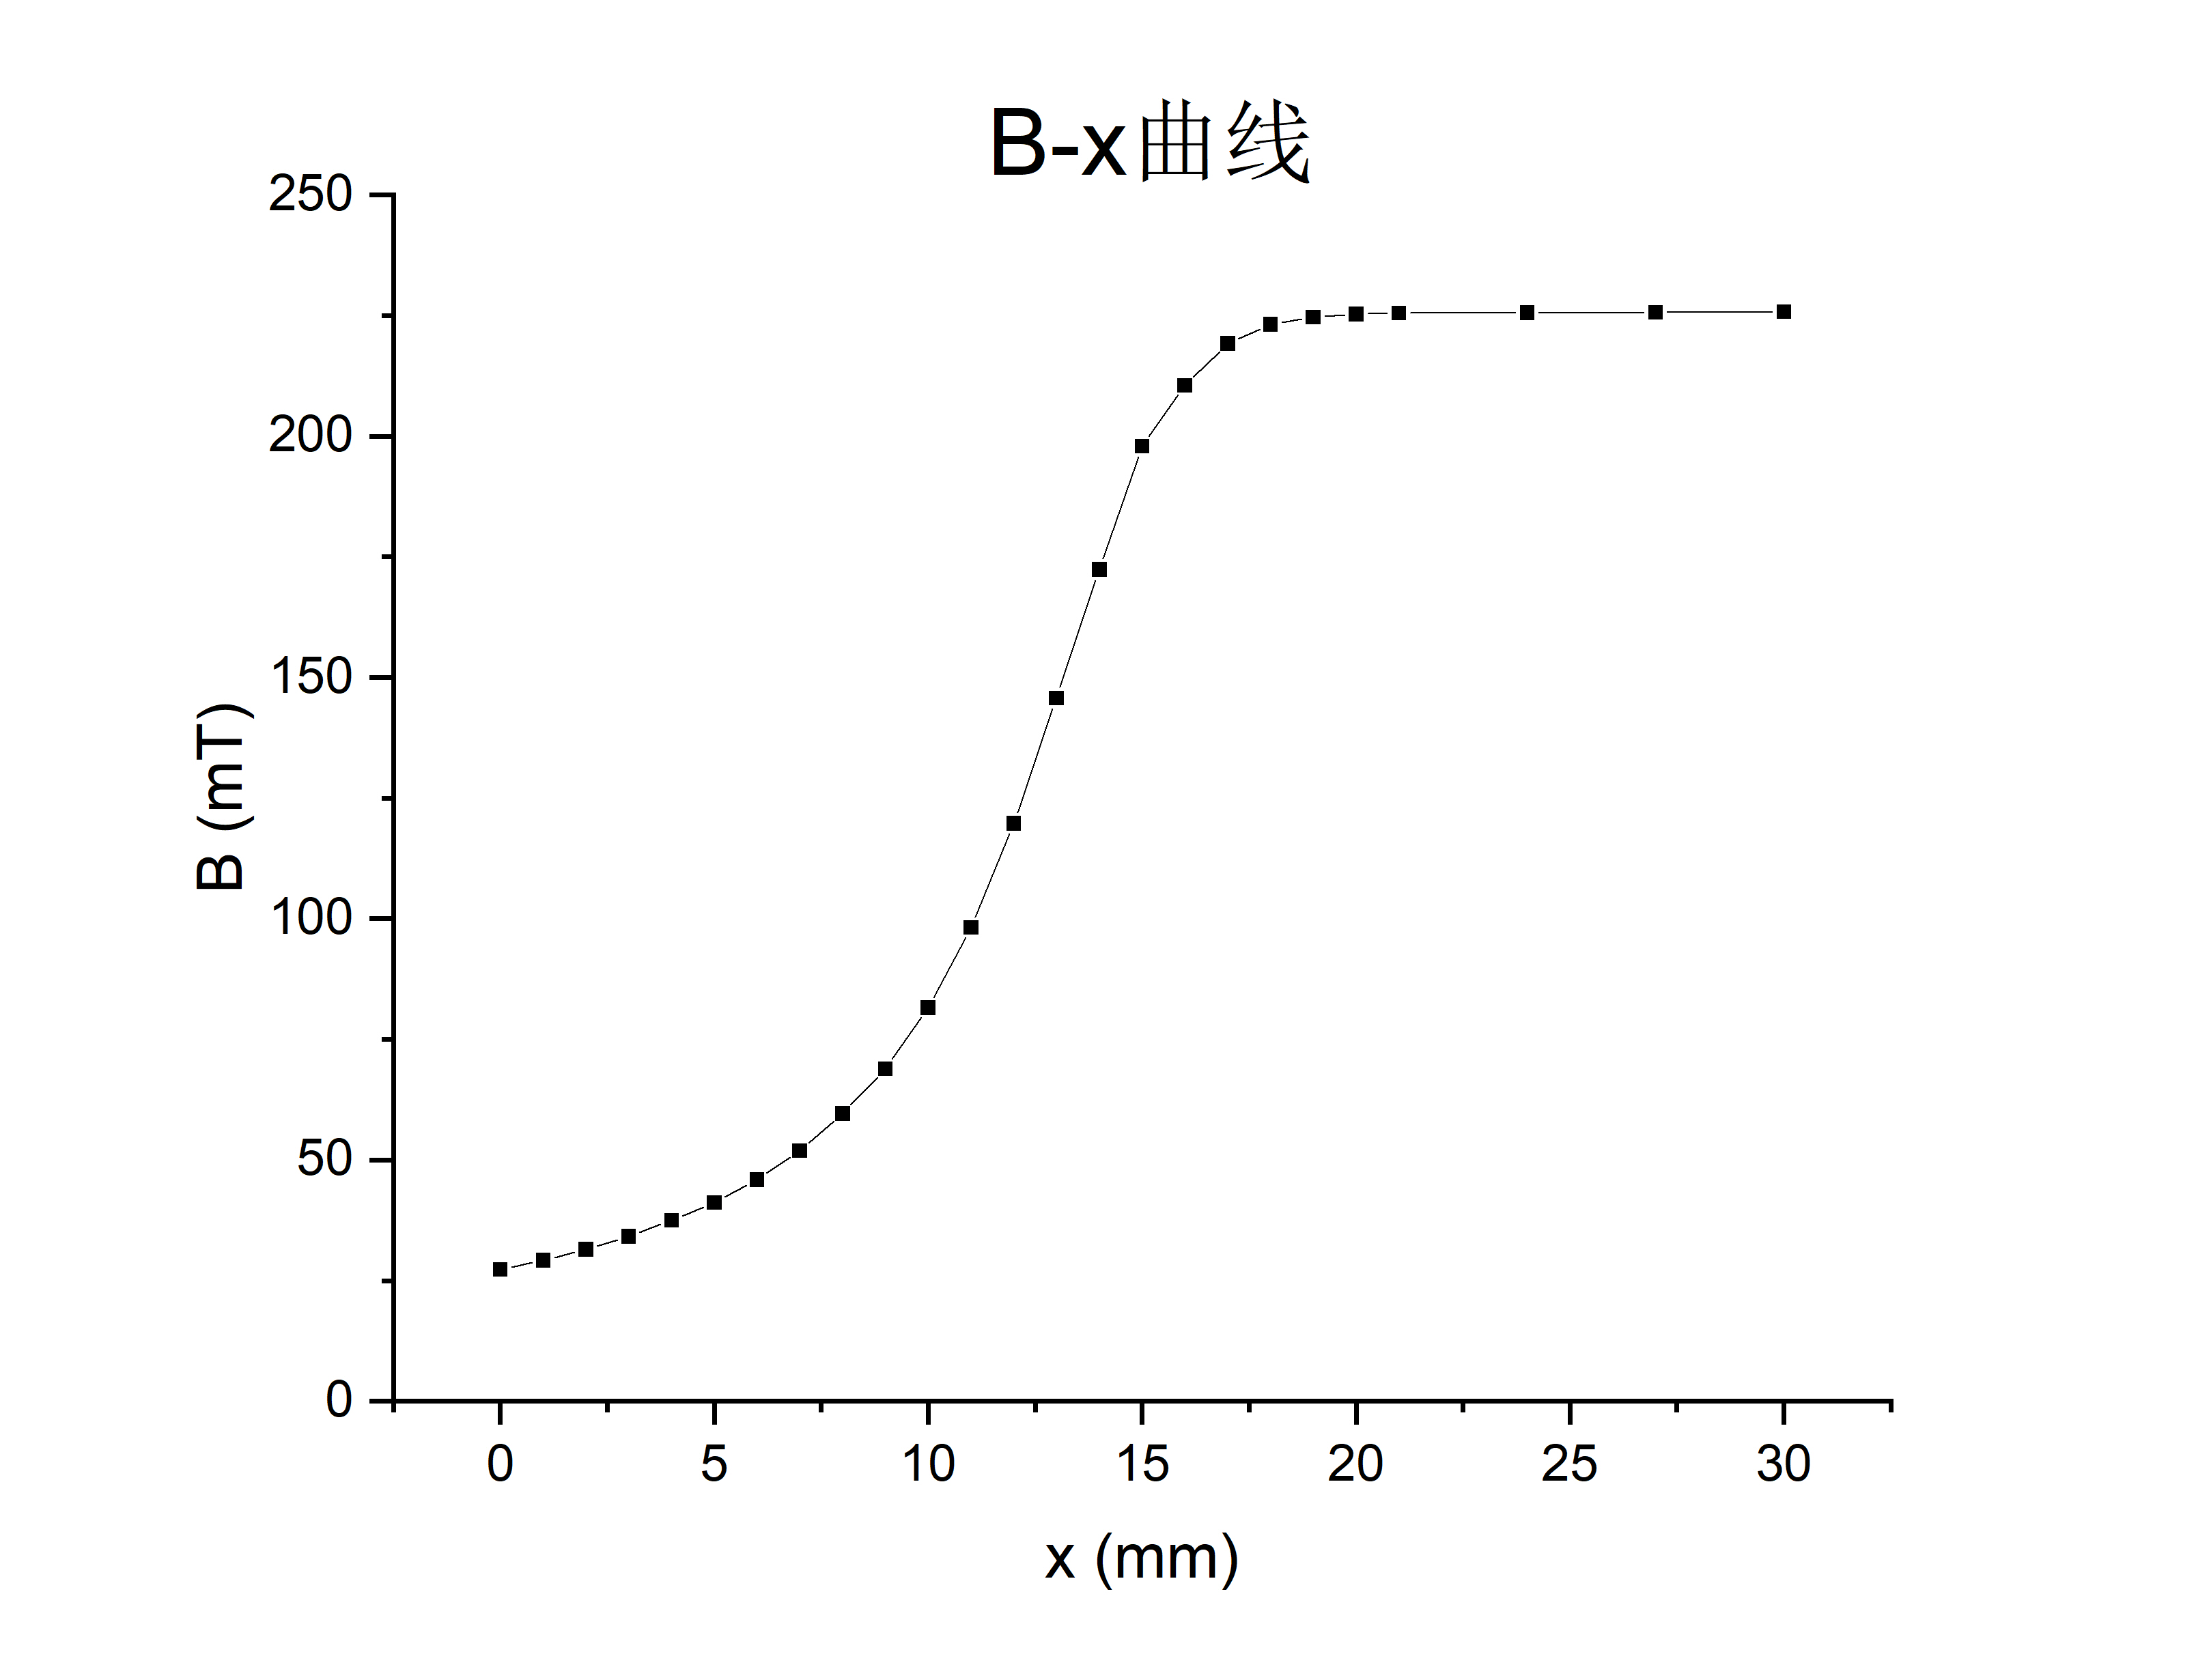
\includegraphics[width=0.8\textwidth]{B-x curve.jpg}
    \end{center}

    根据数据和图线可以看出,在电磁铁的边缘,磁感应强度的大小随着到磁铁中心距离的减小而迅速增大;
    在电磁铁中心附近,磁感应强度大小最大且保持不变。

    \subsection{考察各负效应的值对霍尔电流和外磁场的依赖关系}
    实验中除了霍尔效应,需要考虑的负效应包括埃廷斯豪森效应、能斯特效应、里吉-勒迪克效应和不等位电势差。
    其中霍尔效应产生的霍尔电压$U_H$与电流$I_H$与磁场$B$(方向)有关,埃廷斯豪森效应产生的温差电动势$U_E$也与$U_H$与电流$I_H$与磁场$B$(方向)有关,
    能斯特效应产生的电动势$U_E$与里吉-勒迪克效应产生的电动势$U_R$均与电流$I_H$(方向)无关而与$B$(方向)有关,
    不等位电动势$U_0$则与电流$I_H$(方向)有关而与$B$(方向)无关。因此,可通过以下方法计算负效应的电压值:
    $$U_N+U_R=\frac{1}{4}(U_1+U_2-U_3-U_4)$$
    $$U_0=\frac{1}{4}(U_1-U_2-U_3+U_4)$$
    \subsubsection{各负效应与电流的关系}
    利用实验中从1、2端输入不同电流测得的的数据,分别计算不同霍尔电流下,各负效应的值。实验数据如下表所示:

        \begin{center}
        \begin{tabular}{|c||c|c|c|c||c|c|c|}
            \hline
            $I_M(mA)$ & $U_1(mV)$ & $U_2(mV)$ & $U_3(mV)$ & $U_4(mV)$ & $U(mV)$ & $U_N+U_R(mV)$ & $U_O(mV)$ \\
            \hline
            2.000 & 4.86 & -4.85 & 4.95 & -4.94 & 4.90 & 0.000 & -0.045\\
            \hline
            4.000 & 9.72 & -9.71 & 9.89 & -9.89 & 9.80 & 0.002 & -0.088\\
            \hline
            6.000 & 14.59 & -14.58 & 14.85 & -14.84 & 14.72 & 0.000 & -0.130\\
            \hline
            8.000 &  19.47 & -19.46 & 19.80 & -19.80 & 19.63 & 0.002 & -0.168\\
            \hline
            10.000 & 24.36 & -24.35 & 24.77 & -24.76 & 24.56 & 0.000 & -0.205\\
            \hline
        \end{tabular}        
    \end{center}

    以霍尔电流$I_H$大小为横坐标,不等位电动势$U_0$的绝对值为纵坐标,绘制$U_0-I_H$曲线:

    \begin{center}
        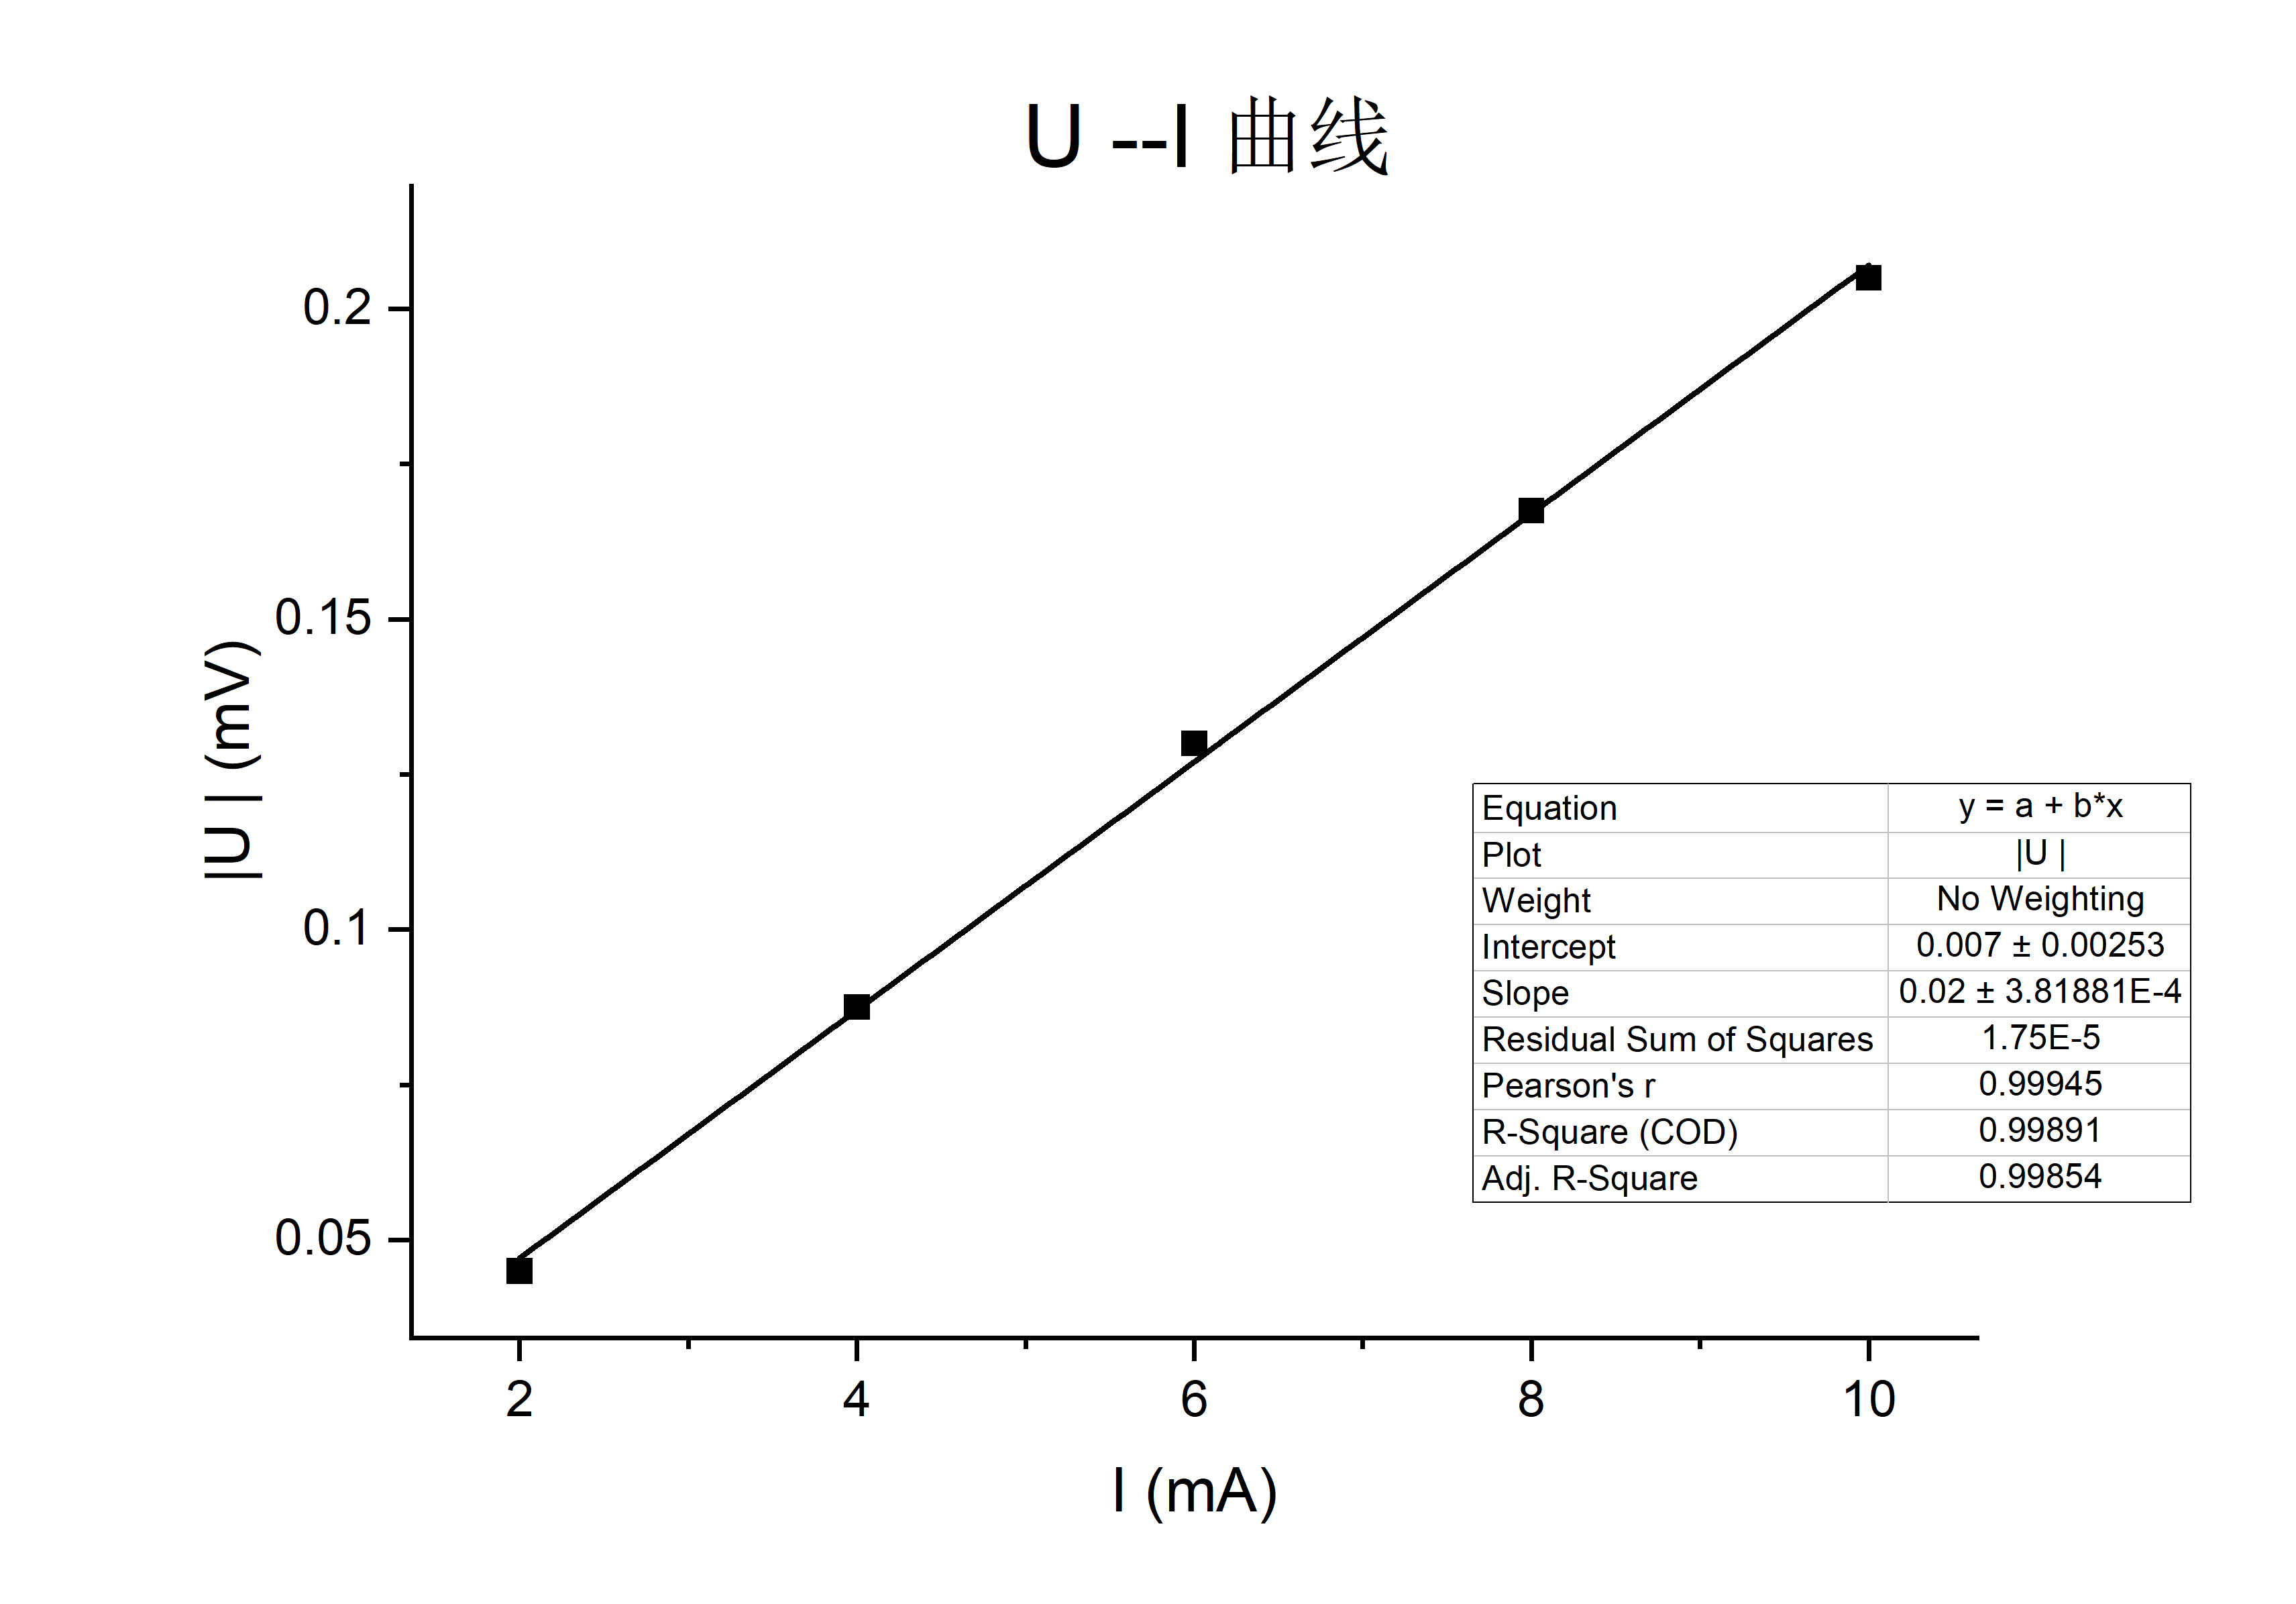
\includegraphics[width=0.8\textwidth]{U0-I curve.jpg}
    \end{center}

    从数据和图线中可以看出,$U_N+U_R$非常小,几乎为0;
    而$U_0$则有一定大小,且其大小与霍尔电流的大小成线性关系。

    \subsubsection{各负效应与外磁场的关系}
    利用实验中从1、2端输入相同电流而改变励磁电流测得的数据,计算各负效应的值:

    \begin{center}
        \begin{tabular}{|c||c||c|c|c|c||c|c|c|}
            \hline
            $I_M(mA)$ & $B(mT)$ &$U_1(mV)$ & $U_2(mV)$ & $U_3(mV)$ & $U_4(mV)$ & $U(mV)$ & $U_N+U_R(mV)$ & $U_O(mV)$\\
            \hline
            0.000 & 1.0 & -0.11 & 0.13 & 0.12 & -0.10 & -0.01  & 0.000 & -0.12\\
            \hline
            0.100 & 36.0 & 3.69 & -3.68 & 4.15 & -4.14 & 3.92 & 0.000 & -0.23 \\
            \hline
            0.200 & 74.9 & 7.89 & -7.89 & 8.38 & -8.37 & 8.13 & -0.003 & -0.24 \\
            \hline
            0.300 & 112.0 & 12.08 & -12.08 & 12.48 & -12.48 & 12.28 & 0.000 & -0.20 \\
            \hline
            0.400 & 151.1 & 16.18 & -16.18 & 16.59 & -16.59 & 16.38 & 0.000 & -0.21 \\
            \hline
            0.500 & 189.0 & 20.23 & -20.22 & 20.72 & -20.72 & 20.47 & 0.003 & -0.25 \\
            \hline
            0.600 & 226.3 & 24.36 & -24.36 & 24.78 & -24.78 & 24.57 & 0.000 & -0.22 \\
            \hline
            0.700 & 266.4 & 28.37 & -28.37 & 28.80 & -28.80 & 28.58  & 0.000 &-0.22\\
            \hline
            0.800 & 298.6 & 32.27 & -32.27 & 32.78 & -32.77 & 32.52 & -0.002 & -0.25 \\
            \hline
            0.900 & 336.6 & 36.23 & -36.23 & 36.66 & -36.66 & 36.44  & 0.000 & -0.22\\
            \hline
            1.000 & 370.4 & 40.01 & -40.00 & 40.45 & -40.43 & 40.22  & -0.003 & -0.22\\
            \hline
        \end{tabular}        
    \end{center}

    从表格中数据可以看出,$U_N+U_R$仍然小得可以忽略不计,$U_O$几乎不随磁场的变化而变化。

    综上,可以得出结论,在实验条件下,$U_N+U_R$可以忽略不计,$U_O$与霍尔电流成正比而与磁场无关。

    \section{思考题}
    思考题(3):在测量$B-I_M$曲线中,$I_M=0$时测量端仍然有较小的电压,这是为什么?

    答:一方面,虽然没有给带磁铁加励磁电流,但磁铁本身带有磁性,会产生一个较小的磁场,造成霍尔效应;
    另一方面,此时霍尔片中是有电流通过的,不等位电势差也会导致测量到较小的电压。
    实验中在消除了不等位电势差等负效应后,测量端电压几乎为0,说明测量端的电压主要是由不等位电势差带来的。

    \section{分析与讨论}
    
    \subsection{比较实验1中a、b两种接法的结果,并解释}
    同一接法下,$U_1,U_2,U_3,U_4$的绝对值基本相等,但仍然可以发现有因负效应带来的差异;
    
    不同接法下,$U_1,U_2,U_3,U_4$有一定差别,但消除负效应后的$U$基本相等,
    这是因为根据霍尔效应的公式$U_H=K_H I_H B=\frac{1}{pqd}I_H B$,霍尔电压只与霍尔片的厚度有关而与长、宽无关。
    两种接法下,霍尔片长、宽虽然不等,但厚度相等,因此霍尔电压相等。

    另外,两种不同接法下,在未消除负效应之前,同一电流、磁场方向的$U$有一定差别,这是因为一些负效应与霍尔片的几何尺寸有关(如非等位电动势)。

    \subsection{说明实验内容3中为什么用计算的$B$作磁化曲线比用直接测量的$B$更好}
    因为实验中直接测量的$B$使用特斯拉计测量的,一方面磁感应强度大小随空间位置的变化而变化,很难精准地测到霍尔片所处位置的磁感应强度大小;
    另一方面,特斯拉计测到的是磁场垂直于其探头霍尔片的分量,所以可能测量到的并不是真实的磁感应强度的大小。
    也就是说,磁场测量的误差要远大于霍尔电压测量的误差。
    
    而用测得的$U_H$和拟合出的$K_H$去计算$B$时,拟合的过程用最小二乘法减小了$B$直接测量所带来的的误差对$K_H$的影响,
    用这两个误差较小的量计算出的$B$自然要比直接测量出的$B$误差要小。

    \subsection{实验中测得的各曲线有何特征?如何理解?}
    $U_H-I_H$、$U_H-B$图线为一直线,说明霍尔电压与霍尔电流、磁感应强度成线性关系。
    
    $B-I$磁化曲线也基本为一直线,这反映了实验所使用的的电磁铁材料的性质。
    
    $B-x$曲线为一缓慢上升-快速上升-缓慢上身-保持不变的曲线,说明在电磁铁边缘位置,磁感应强度随着到中心距离的减小而迅速增加,
    在电磁铁中心附近,磁感应强度大小最大且保持不变。

    \section{收获与感想}
    本次实验收获最大的是实验中所使用的到的消除负效应的方法:根据各效应与电流、磁场的关系,改变电流磁场方向进行测量,
    对测的结果进行运算来消除负效应。在其他实验中可能也会遇到类似的负效应影响实验结果,在这种情况下可以类比本实验,
    通过考察其对某些物理量的依赖关系(尤其是正负对某些物理量方向的依赖关系),通过对直接测量结果进行代数运算,消除负效应,
    间接测量需要的物理量。
\end{document}